
\documentclass[12pt,t]{beamer}
\usepackage[utf8]{inputenc}
\usepackage{graphicx}
%\usepackage{amssymb,amsmath}
%\usepackage{verbatim} 
%\usepackage{url}
%\usepackage{float}
%\usepackage{color}
%\usepackage{listings}
%\usepackage{hyperref}
%\usepackage{subfig}
%\usepackage{pslatex}
\usetheme[unit=ics,dk]{Frederiksberg}
\title{Detektion af vesikler i celler}
\subtitle{Bachelorforsvar}
\author{Claes Nøhr Ladefoged \and \\
Marcus Bjerg Gregersen}
\institute{Datalogisk Institut}
\date[]{20. Juni 2011}
\begin{document}
\frame[plain]{\titlepage}

\begin{frame}
\frametitle{Intro}
\begin{itemize}
	\item Argument 1 
	\item Argument 2
	\item Killer Argument!
\end{itemize}
\end{frame}

\begin{frame}
\frametitle{Intro fortsat}
Det er smart fordi....
\begin{figure}[H]
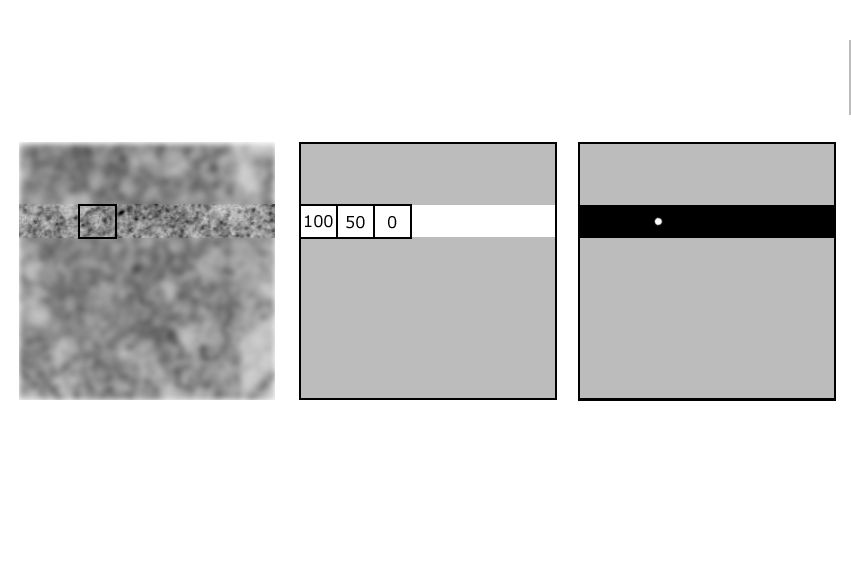
\includegraphics{9.png}
\end{figure}
\end{frame}
\end{document}
